\documentclass[11pt,letterpaper]{article}
\usepackage[margin=1in]{geometry}
\usepackage{fontspec}
\usepackage{microtype,booktabs,graphicx,amsmath,longtable,array}
\usepackage[round,authoryear]{natbib}
\usepackage[font=small,labelfont=bf]{caption}
\usepackage[hidelinks]{hyperref}
\usepackage{xurl,setspace}
\setstretch{1.15}
\setlength{\emergencystretch}{2em}
\newcommand{\Classified}{157}
\newcommand{\ClassifiedFlagged}{79}
\newcommand{\ClassifiedComparison}{78}
\newcommand{\Covered}{155}
\newcommand{\Analyzed}{153}
\newcommand{\Flagged}{76}
\newcommand{\Comparison}{77}
\newcommand{\Serious}{43}
\newcommand{\ZeroYears}{29}
\newcommand{\Records}{16,437}
\newcommand{\Repaired}{1}
\newcommand{\Duplicates}{15}
\newcommand{\FalseLinks}{3}
\newcommand{\Prepublication}{54}
\newcommand{\MainEstimate}{1.8}
\newcommand{\MainLower}{-2.1}
\newcommand{\MainUpper}{5.7}
\newcommand{\MainLoss}{2.1}
\newcommand{\MainInterval}{[-2.1, 5.7]}
\newcommand{\FlaggedBefore}{9.4}
\newcommand{\FlaggedAfter}{21.4}
\newcommand{\ComparisonBefore}{6.5}
\newcommand{\ComparisonAfter}{16.7}
\newcommand{\FlaggedChange}{11.9}
\newcommand{\ComparisonChange}{10.1}
\newcommand{\AdjustedEstimate}{0.8}
\newcommand{\AdjustedInterval}{[-2.8, 4.4]}
\newcommand{\InclusiveEstimate}{1.6}
\newcommand{\InclusiveInterval}{[-2.3, 5.5]}
\newcommand{\SeriousEstimate}{4.3}
\newcommand{\SeriousInterval}{[-0.1, 8.7]}
\newcommand{\PretrendEstimate}{4.3}
\newcommand{\PretrendInterval}{[0.1, 8.6]}
\newcommand{\BootstrapLower}{-2.0}
\newcommand{\BootstrapUpper}{5.6}
\newcommand{\BootstrapDraws}{9,999}
\newcommand{\BootstrapSeed}{31415}
\newcommand{\LeaveMin}{1.3}
\newcommand{\LeaveMax}{2.5}
\newcommand{\SharedPercent}{13.7}
\newcommand{\CodingN}{100}
\newcommand{\Rated}{95}
\newcommand{\Ack}{1}
\newcommand{\Nonack}{94}
\newcommand{\AckPercent}{1.1}
\newcommand{\AckLower}{0.2}
\newcommand{\AckUpper}{5.7}
\newcommand{\AckBoundLower}{1.0}
\newcommand{\AckBoundUpper}{3.1}
\newcommand{\Uncoded}{1}
\newcommand{\Unavailable}{1}
\newcommand{\CodingFalse}{3}
\newcommand{\PartialYear}{7}

\title{Significant Error:\\Citations to Research With Publicized Statistical Errors}
\author{Ken Cor \and Gaurav Sood}
\date{October 2026}
\hypersetup{pdfauthor={Ken Cor and Gaurav Sood},pdftitle={Significant Error: Citations to Research With Publicized Statistical Errors}}
\begin{document}
\maketitle
\begin{abstract}
\noindent Does drawing attention to a statistical mistake change how researchers use papers containing it? A 2011 critique in \textit{Nature Neuroscience} explained a common mistake: inferring that two effects differ because one is statistically significant and the other is not. Using classifications supplied by the critique's authors, we compare citation patterns for papers that made the mistake and papers that used the relevant test correctly. Flagged papers continued to attract citations. From 2010 to the annual average for 2012--2015, citations increased by \FlaggedChange{} per flagged paper and \ComparisonChange{} per comparison paper, a difference of \MainEstimate{} (95\% interval \MainInterval). In a separate sample of citing articles, \Nonack{} of \Rated{} valid completed ratings recorded no acknowledgment of concerns. These findings show continued use of affected papers with little recorded acknowledgment. They do not establish that publicity had no effect: citation growth already differed before the critique, and the records do not reveal whether citing authors recognized the mistake or relied on a conclusion it undermined.
\end{abstract}
\vspace{1em}
\noindent\small We thank Danielle Portnoy and Xiaoran Huang for research assistance, and Andrew Gelman, Kabir Khanna, and Daniel Stone for comments. Replication materials: \url{https://github.com/recite/sig_fault}.\normalsize

\newpage
\section{Introduction}
Scientific articles build on findings reported by others. When those findings rest on faulty reasoning, later citations can carry the mistake forward. Retraction is one signal that a paper should be treated with caution, but statistical errors also occur in papers that remain part of the published literature. Researchers may recognize such errors themselves, especially after a methodological critique draws attention to them. Whether that recognition changes subsequent use of the affected research is an empirical question.

One recurring mistake is to treat a statistically significant effect in one group and a nonsignificant effect in another as evidence that the groups differ. That conclusion requires a test of the difference itself. Significance in one group can reflect greater precision rather than a larger effect \citep{gelman2006}. Failure to test the difference leaves the claimed contrast unsupported by that argument; it does not establish that the underlying effects are equal or that every conclusion in the paper is false.

\citet{nieuwenhuis2011} documented the problem in neuroscience research. Their review identified \Classified{} papers in which a comparison of effects was relevant and classified \ClassifiedFlagged{} as making the mistake. They supplied us with the paper-level classifications. Those records let us follow the affected papers and compare their citations with those of papers in the review that used the appropriate test.

Our hypothesis is that papers containing the mistake receive fewer subsequent citations relative to comparison papers after the critique appears. Researchers who understand the critique can inspect the original analyses and reconsider whether to rely on them. They might instead continue to cite the paper while qualifying the affected finding. We therefore examine both citation rates and whether citing papers acknowledge concerns.

A general methodological warning can change how readers evaluate particular studies by making the mistake easier to recognize. The response depends on whether researchers encounter the warning, recognize the mistake, and regard it as consequential for the claim they wish to support. Citation records reveal the resulting use of a paper, not each of these steps. This distinction matters when interpreting continued citation.

\section{Data and research design}
\subsection{Source papers and citation histories}
The source review covers behavioral, systems, and cognitive neuroscience papers published in 2009--2010 in \textit{Nature}, \textit{Science}, \textit{Nature Neuroscience}, \textit{Neuron}, and sampled issues of the \textit{Journal of Neuroscience}. We use its classification of whether a paper made the particular statistical mistake, rather than attempting a new assessment of each scientific result. ``Comparison'' consequently means no such mistake in the reviewed analysis, not freedom from all possible errors.

The local citation exports cover \Covered{} of the \Classified{} classified papers. Two have no exported history and are excluded rather than assigned zero citations. Two further histories contain the target paper itself and records published before it, indicating that the exported lists are not valid citing-article searches. The main analysis excludes those histories, leaving \Flagged{} flagged and \Comparison{} comparison papers. Appendix~\ref{app:data} describes the checks, and Table~\ref{tab:sensitivity} reports the estimate with the two histories retained.

The outcome is the number of distinct citing documents recorded for a paper in a calendar year. We collapse duplicate records for the same cited paper using DOI where available and database accession otherwise. A document citing several study papers contributes to each paper's count. We repair a malformed export row and remove the false citation links explicitly identified in the archived coding. All original source files remain in the replication materials.

For every covered paper we retain years with no citation records and assign a count of zero. These are zeros within an available export, not a claim that the database captures every citation in the world. The descriptive series runs from 2009 through 2015. The export was saved in April 2016, so that year's incomplete counts are excluded from the rate analysis.

\subsection{Timing and comparison}
The critique appeared online on August 26, 2011 \citep{nieuwenhuis2011}. Our baseline is 2010, the last full calendar year before its publication, and the post-critique period is 2012--2015. We omit 2011 from the main before--after contrast because it combines months before and after publication. The first citation counts after publicity can also include manuscripts written or accepted earlier. We therefore examine later windows while keeping the baseline fixed.

Let $C_{it}$ be citations to paper $i$ in year $t$, and let $F_i$ indicate a paper flagged for the mistake. We calculate each paper's change,
\[
 D_i = \frac{1}{4}\sum_{t=2012}^{2015} C_{it} - C_{i,2010},
\]
and compare the mean changes:
\[
 \widehat\delta = \overline D_{F=1} - \overline D_{F=0}.
\]
A negative value is the relative decline predicted by our hypothesis. The unit is additional citations per paper per year; each source paper receives equal weight. Comparing annual averages avoids treating a longer post-critique observation window as evidence of increased citation rates.

This is a difference-in-differences comparison. Interpreting it as the critique's effect requires the groups to have followed comparable changes in citation rates without the critique. Papers making the mistake may differ in topic, prominence, findings, and ordinary citation growth. Publication in the same journals and years helps define a relevant comparison but does not guarantee comparable trajectories. Both groups can be affected by a general methodological warning, so any causal interpretation would concern a differential response, not the critique's total influence on research.

We report a Welch confidence interval over paper-level changes, allowing different variances in the two groups. Collapsing each paper to its before--after change keeps its repeated annual counts together. The interval treats papers as independent units; common topics and shared citing documents may introduce dependence across papers. We use it as model-based uncertainty for the comparison, not as a randomized-treatment interval or a correction for confounding. Appendix~\ref{app:inference} reports influence and bootstrap checks.

\section{Citation patterns}
\subsection{Continued citation and changes relative to comparison papers}
Citation rates rose in both groups as these recently published papers accumulated attention (Figure~\ref{fig:paths}). Flagged papers averaged \FlaggedBefore{} citations in 2010 and \FlaggedAfter{} per year in 2012--2015. Comparison papers increased from \ComparisonBefore{} to \ComparisonAfter{} (Table~\ref{tab:levels}). Continued citation is therefore clear, but an increase by itself does not demonstrate that the critique failed: citations might have grown still more without it.

\begin{figure}[htbp]
\centering
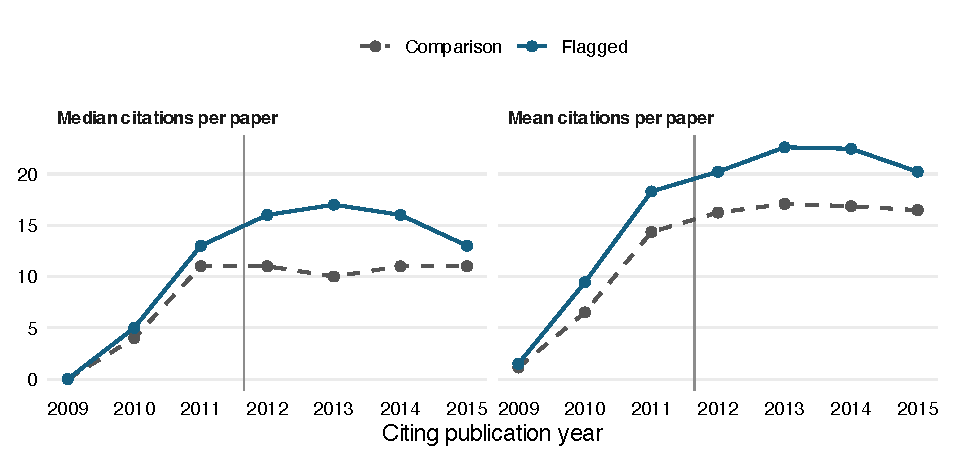
\includegraphics[width=\linewidth]{../figs/citation_paths.pdf}
\caption{Citation trajectories for \Flagged{} flagged and \Comparison{} comparison papers. Lines show observed annual means and medians, including years with no recorded citations. The vertical line marks August 2011, when the critique appeared. These are descriptive summaries of the included papers, without sampling intervals. The 2009 series includes prepublication zeros for the papers published in 2010; the main comparison uses 2010 as its baseline.}
\label{fig:paths}
\end{figure}

\begin{table}[htbp]
\centering
\caption{Mean annual citations before and after the critique}
\label{tab:levels}
\begin{tabular}{lrrrr}
\toprule
Article group & Papers & 2010 & 2012--2015 & Change \\
\midrule
Flagged & 76 & 9.4 & 21.4 & 11.9 \\
Comparison & 77 & 6.5 & 16.7 & 10.1 \\
\bottomrule
\end{tabular}

\par\smallskip
\begin{minipage}{.95\linewidth}\footnotesize
2012--2015 is the annual average over that period. Change is the post-period average minus 2010. Each source paper has equal weight. The difference between group changes is \MainEstimate{} citations per paper per year, with a 95\% Welch interval of \MainInterval.
\end{minipage}
\end{table}

The flagged group gained \FlaggedChange{} annual citations per paper, compared with \ComparisonChange{} for the comparison group. The difference, \MainEstimate{} (95\% interval \MainInterval), runs opposite to the predicted decline. Its uncertainty nevertheless allows a relative reduction of roughly \MainLoss{} citations per paper per year as well as a larger increase. We cannot equate an imprecise positive estimate with evidence that publicity had no effect.

The earlier trajectory further limits a causal reading. Among papers published in 2009, the flagged group's increase from 2009 to 2010 was already \PretrendEstimate{} citations larger (95\% interval \PretrendInterval). The publication year is a short and uneven exposure window, so this is not a definitive test of what later trends would have been. It does show that equal growth cannot simply be assumed. We have too little comparable pre-critique history to establish a persuasive counterfactual trajectory.

\subsection{Alternative comparisons}
Adjusting the paper-level changes for journal and publication year gives a difference of \AdjustedEstimate{} (95\% interval \AdjustedInterval). Retaining the two questionable histories gives \InclusiveEstimate{} (\InclusiveInterval). Neither data cleaning nor this adjustment produces the predicted relative decline, but the adjustment cannot remove unmeasured differences in papers' citation trajectories.

Later post-critique windows also yield positive point estimates, with considerable uncertainty (Table~\ref{tab:sensitivity}). These comparisons allow more time for citing manuscripts to respond; they do not redefine early post-critique years as untreated years. Year-specific comparisons are shown in Appendix~\ref{app:inference}.

The original reviewers also described some errors as ``potentially serious.'' Their notes express uncertainty about the consequences of the missing test; they do not establish that the main findings would fail under a correct analysis. Comparing the \Serious{} included papers with that classification against the same \Comparison{} comparison papers gives a difference of \SeriousEstimate{} (95\% interval \SeriousInterval). Other flagged papers do not enter this comparison group.

\section{Acknowledgment in citing papers}
Researchers can respond to a problematic finding by qualifying it rather than withholding a citation. The archived citation-context sample lets us examine that response. It contains \CodingN{} citation relationships selected after 2011, including \PartialYear{} from the incomplete 2016 export. This sample therefore has a slightly longer window than the annual citation analysis.

The available file contains \Rated{} completed ratings of valid citation relationships: \Nonack{} record no acknowledgment of concerns, and \Ack{} records acknowledgment. The remaining records comprise \CodingFalse{} false citation links, \Unavailable{} article that could not be located, and \Uncoded{} record with no completed rating. Among valid completed ratings, the acknowledgment share is \AckPercent\% (95\% Wilson interval [\AckLower, \AckUpper]\%). Assigning both unresolved, non-false records to either category puts that share between \AckBoundLower\% and \AckBoundUpper\% among all non-false sampled relationships. These bounds concern missing coding, not sampling uncertainty.

This finding describes recorded acknowledgment. The coding protocol counts acknowledgment of any concern about the cited paper, not only the specific interaction error. Absence of a concern does not establish that the citation endorses the faulty inference: a paper may be cited for a different finding, a method, or background. Nor does it reveal whether the citing authors noticed the mistake and judged it unimportant. The distinction between recognizing an error and changing citation behavior remains unresolved.

\section{Discussion}
The affected papers remained in use after a prominent critique explained their statistical mistake. Their citations did not show the predicted decline relative to the comparison papers, and explicit acknowledgment of concerns was rare in the archived coding.

The evidence is weaker about the critique's causal effect. Citation growth differed before publication, individual awareness is unobserved, and some citations could have been committed to print before the warning appeared. A warning could reduce reliance on a faulty claim while total citations to its paper continue to grow. Conversely, continued unqualified use of the faulty claim would be consistent with failure to recognize or act on the problem. Citation totals and the available context codes cannot distinguish these possibilities.

The practical implication is a question about how criticism reaches the point of use. Methodological critiques give readers the tools to recognize a mistake, but doing so requires them to connect that guidance to an analysis in another paper. Linking methodological concerns to specific findings could make that assessment easier. Establishing whether such links improve citation practice would require a design that measures or varies exposure and distinguishes use of the affected finding from other reasons to cite the paper.

\bibliographystyle{plainnat}
\bibliography{references}

\clearpage
\appendix
\section{Data construction and citation-context records}\label{app:data}
The supplied classification spreadsheet identifies the articles by journal, publication year, page, and study characteristics. The identified Excel and CSV versions agree on the paper-level YES/NO codes. The citation import reads \Records{} database records across the covered sheets, repairs \Repaired{} malformed record, and marks \Duplicates{} duplicate DOI records within cited papers. It removes \FalseLinks{} citation relationships identified as false in the historical context coding. Full source hashes and record-level indicators are generated by the replication scripts.

The unreliable histories are source IDs 23 and 25. Matching the intended papers' journal, year, and supplied page locates the target papers themselves in their supposed citing-article exports. Those histories also contain \Prepublication{} records before the target publication year. This combination is consistent with exporting literature-search results instead of the intended citation results. The saved workbook contains no query log with which to reconstruct the precise operation. Deleting only the early records would not establish the validity or completeness of the remaining links. The principal estimates exclude both histories, while the inclusive estimate shows the effect of retaining them. The other sheets contain neither a target-self match nor a record before the target year under these checks.

Missing sheets, source IDs 95 and 124, remain missing. In covered histories the completed 2010--2015 panel includes \ZeroYears{} paper-years with zero recorded citations. The scripts check that every paper has each required year and that joining the classification does not multiply or discard citation records.

\begin{table}[htbp]
\centering
\caption{Disposition of the historical citation-context sample}
\label{tab:coding}
\begin{tabular}{lr}
\toprule
Recorded status & Citation relationships \\
\midrule
Article unavailable &  1 \\
Concern recorded &  1 \\
False citation link &  2 \\
No concern recorded & 95 \\
Uncoded &  1 \\
\bottomrule
\end{tabular}

\par\smallskip
\begin{minipage}{.95\linewidth}\footnotesize
The sample consists of citation relationships from 2012 through the partial 2016 export. Every relationship matches a record in the source workbooks. ``No concern recorded'' and ``Concern recorded'' reproduce completed historical codes for valid citation relationships. The other categories preserve missingness and known false links.
\end{minipage}
\end{table}

The original coding protocol instructed the rater to assess whether a citing paper noted concerns about the cited paper, using the citing text and original article. The distributed file contains the rating and selected contextual text, not the full highlighted PDFs. We retain those ratings rather than claiming to have independently recoded the articles. The available materials contain one set of item-level ratings, so intercoder agreement cannot be independently checked.

\section{Sensitivity and uncertainty}\label{app:inference}
Table~\ref{tab:sensitivity} reports the full set of specified comparisons. The cohort and potentially-serious-error rows describe restricted populations. The pre-critique row is a diagnostic, not an estimate of the critique's effect. All choices were made retrospectively; these are not preregistered confirmatory tests.

\begin{table}[htbp]
\centering
\caption{Differences in citation changes under alternative comparisons}
\label{tab:sensitivity}
\small
\begin{tabular}{p{7.0cm}rrr}
\toprule
Comparison & Flagged / other & Difference & 95\% interval \\
\midrule
Main comparison & 76 / 77 & 1.8 & [-2.1, 5.7] \\
Journal and publication-year adjustment & 76 / 77 & 0.8 & [-2.8, 4.4] \\
Retain both questionable citation histories & 78 / 77 & 1.6 & [-2.3, 5.5] \\
Retain duplicate database records & 76 / 77 & 1.8 & [-2.2, 5.7] \\
Retain known false citation links & 76 / 77 & 1.8 & [-2.1, 5.7] \\
Papers published in 2009 & 44 / 47 & 2.5 & [-2.3, 7.4] \\
Papers published in 2010 & 32 / 30 & 0.3 & [-6.4, 7.0] \\
Later window: 2013-2015 & 76 / 77 & 2.0 & [-2.2, 6.2] \\
Later window: 2014-2015 & 76 / 77 & 1.7 & [-2.5, 6.0] \\
Potentially serious errors only & 43 / 77 & 4.3 & [-0.1, 8.7] \\
Pre-critique change: 2009 cohort, 2009 to 2010 & 44 / 47 & 4.3 & [0.1, 8.6] \\
\bottomrule
\end{tabular}

\par\smallskip
\begin{minipage}{\linewidth}\footnotesize
Differences are flagged minus comparison, in citations per paper per year. Except for the final row, the baseline is 2010; the post period is 2012--2015 unless another window is named. Intervals are pointwise 95\% Welch intervals, except the journal/year-adjusted estimate, which uses OLS with HC3 standard errors and a residual-degrees-of-freedom $t$ critical value. The final row compares 2010 with 2009 among papers published in 2009.
\end{minipage}
\end{table}

Citation counts are skewed, so we retain the mean as the estimand and separately display medians in Figure~\ref{fig:paths}. Removing each source paper in turn gives main point estimates from \LeaveMin{} to \LeaveMax. A stratified bootstrap that resamples whole papers within the flagged and comparison groups gives a percentile interval of [\BootstrapLower, \BootstrapUpper]. The replication uses \BootstrapDraws{} draws and seed \BootstrapSeed. Both this bootstrap and the Welch interval treat papers as independent; neither addresses a common omitted determinant of their citation trajectories.

Of the distinct citing documents in the main papers' 2010--2015 records, \SharedPercent\% cite more than one study paper. Shared citing documents and related research topics can connect citation counts across source papers. The reported intervals do not model those connections. The data are also a selected set of papers from particular journals and years, so the numerical comparison is not a probability-sample estimate for all scientific publishing.

\begin{figure}[htbp]
\centering
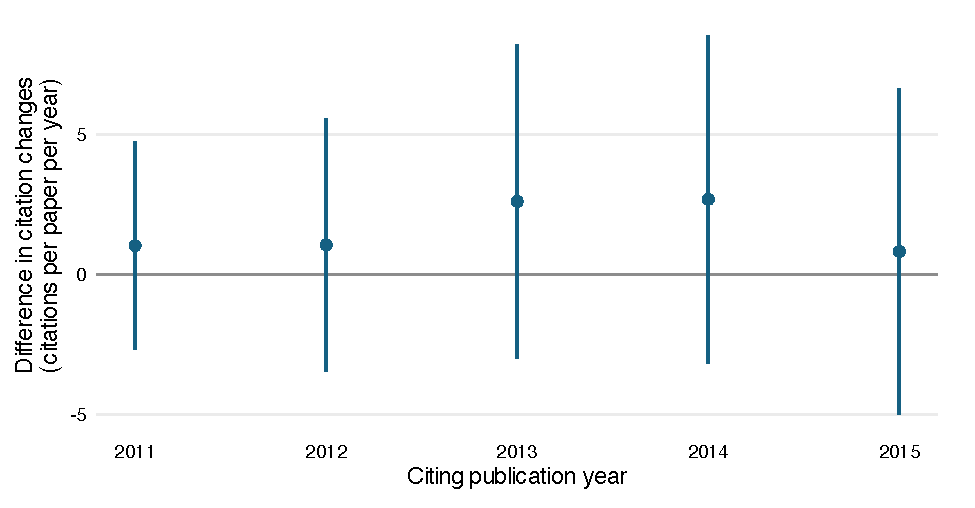
\includegraphics[width=\linewidth]{../figs/year_contrasts.pdf}
\caption{Year-specific changes from 2010, flagged minus comparison. Points compare changes for the same \Flagged{} flagged and \Comparison{} comparison papers. Bars are simultaneous 95\% Bonferroni intervals for the five displayed contrasts, using Welch standard errors and degrees of freedom. The 2011 point describes the transition year and is excluded from the main post-period average. The zero line denotes equal changes in citation rates.}
\label{fig:years}
\end{figure}
\end{document}
